\documentclass[tikz,border=4pt]{standalone}
\usepackage{amsmath,amssymb}
\usetikzlibrary{positioning,arrows.meta,calc,fit}
\begin{document}
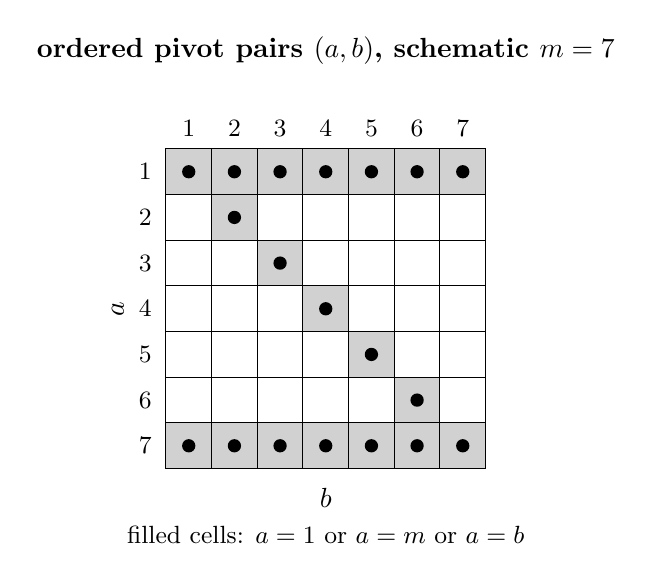
\begin{tikzpicture}[x=.58cm,y=.58cm,font=\small]
\node[font=\bfseries] at (4.5,1.15) {ordered pivot pairs $(a,b)$, schematic $m=7$};
% Grid with a increasing downward, b increasing rightward.
\foreach \a in {1,...,7}{
  \foreach \b in {1,...,7}{
    \draw (\b,-\a) rectangle +(1,-1);
  }
}
% Compatibility: a=1 or a=m or a=b.
\foreach \b in {1,...,7}{
  \fill[black!18] (\b,-1) rectangle +(1,-1);
  \fill[black!18] (\b,-7) rectangle +(1,-1);
  \fill (\b+.5,-1.5) circle (2.4pt);
  \fill (\b+.5,-7.5) circle (2.4pt);
}
\foreach \a in {1,...,7}{
  \fill[black!18] (\a,-\a) rectangle +(1,-1);
  \fill (\a+.5,-\a-.5) circle (2.4pt);
}
% Redraw cell borders over fills.
\foreach \a in {1,...,7}{\foreach \b in {1,...,7}{\draw (\b,-\a) rectangle +(1,-1);}}
% Tick labels.
\foreach \i in {1,...,7}{
  \node at (\i+.5,-.55) {$\i$};
  \node at (.55,-\i-.5) {$\i$};
}
\node[font=\bfseries] at (4.5,-8.65) {$b$};
\node[font=\bfseries,rotate=90] at (-.05,-4.5) {$a$};
\node[align=center] at (4.5,-9.45) {filled cells: $a=1$ or $a=m$ or $a=b$};
\end{tikzpicture}
\end{document}
